\documentclass{article}
\usepackage{parskip}
\usepackage{amsmath}
\usepackage{graphicx}
\graphicspath{ {./} }
\usepackage{tikz}
\usetikzlibrary{shapes.geometric, arrows, plotmarks}
\tikzstyle{startstop} = [rectangle, rounded corners, minimum width=3cm, minimum height=1cm, text centered, draw=black]
\tikzstyle{process} = [rectangle, minimum width=3cm, minimum height=1cm, text centered, draw=black]
\tikzstyle{decision} = [diamond, aspect=2, minimum width=3cm, minimum height=1cm, text centered, draw=black]
\tikzstyle{arrow} = [thick,->,>=stealth]
\usepackage{float}

\setlength{\belowcaptionskip}{10pt}

\title{Project 1: Search for Intelligent Puzzles}
\author{John Bradley}
\date{\today}

\begin{document}
  \maketitle

  \section{Introduction}

  This report aims to document the implementation and analysis of a 
  bag-of-tasks model similar to that of the SETI@Home program. The program
  is split into a server-client relationship where a SETI server sends data to
  a client located somewhere in the world. The data involved in the transaction
  is relatively small compared to the computational requirements, and each task
  is independent of each other. This project's goal is to search for 
  "intelligent puzzles", or solvable game states of a peg hopping game.  This 
  report will cover the methods and techniques utilized for implementing the 
  bag-of-tasks model, analyze and estimate the expected performance of the 
  implementation, present the results from experimentation, compare and contrast 
  the expected performance to the observed results, and conclude with insights 
  and possible changes that could be made to the implementation.

  \section{Methods and Techniques}

  The method of determining a solvable game state is given to us and is not the
  focus of the implementation, and thus can be considered a "black box", where
  the specifics aren't discussed in detail. Instead, the distribution of tasks,
  or initial game states to be solved, will be covered.

  In order to minimize communication costs, the tasks will be grouped and sent
  to the client when a client indicates that it is ready for a packet of data
  to process. These packets will be of limited size in order to allow for faster
  clients to process more packets as needed.

  As there may be some time where the server is idle, such as waiting for a
  packet of results from clients, and this idle time can be better utilized to
  process additional game states. The number of games that the server processes
  will be \(\frac{n}{2}\), where \(n\) is the size of packet being sent to clients.
  This packet size can be varied, and will be discussed later in this section.

  \begin{figure}[t]
    \caption{Server Logic Flow}
    \label{fig:serverflow}
    \centering

    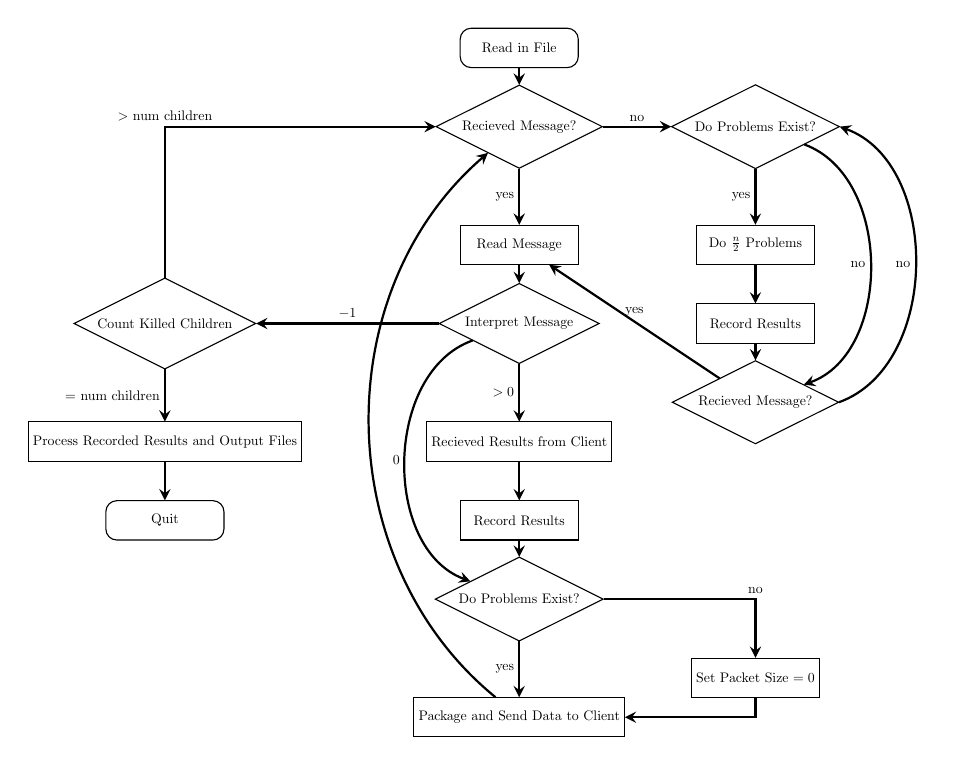
\begin{tikzpicture}[node distance=2cm, every node/.style={scale=0.5}, tips=proper]
      \node (start)    [startstop, yshift=-1cm]                    {Read in File};
      \node (dcrecv)   [decision,  below of=start]                 {Recieved Message?};
      \node (crecv2)   [process,   below of=dcrecv, yshift=-1cm]   {Read Message};
      \node (dimsg)    [decision,  below of=crecv2]                {Interpret Message};
      \node (crecv3)   [process,   below of=dimsg, yshift=-1cm]    {Recieved Results from Client};
      \node (srec1)    [process,   below of=crecv3]                {Record Results};
      \node (dsprob1)  [decision,  below of=srec1]                 {Do Problems Exist?};
      \node (pkgsend)  [process,   below of=dsprob1, yshift=-1cm]  {Package and Send Data to Client};

      \node (dcntkc)   [decision,  left of=dimsg, xshift=-7cm]     {Count Killed Children};
      \node (presult)  [process,   below of=dcntkc, yshift=-1cm]   {Process Recorded Results and Output Files};
      \node (stop)     [startstop, below of=presult]               {Quit};

      \node (dsprob2)  [decision,  right of=dcrecv, xshift=4cm]    {Do Problems Exist?};
      \node (swork)    [process,   below of=dsprob2, yshift=-1cm]  {Do \(\frac{n}{2}\) Problems};
      \node (srec2)    [process,   below of=swork]                 {Record Results};
      \node (dcrecv2)  [decision,  below of=srec2]                 {Recieved Message?};

      \node (setpkt)   [process,   below of=dcrecv2, yshift=-5cm]  {Set Packet Size \(=0\)};

      \draw [arrow] (start)   -- (dcrecv);
      \draw [arrow] (dcrecv)  -- node[anchor=east]  {yes}     (crecv2);
      \draw [arrow] (dcrecv)  -- node[anchor=south] {no}      (dsprob2);
      \draw [arrow] (crecv2)  -- (dimsg);
      \draw [arrow] (dimsg)   -- node[anchor=east]  {\(>0\)}  (crecv3);
      \draw [arrow] (dimsg)   edge[bend right=70] node[anchor=east] {\(0\)}  (dsprob1);
      \draw [arrow] (dimsg)   -- node[anchor=south] {\(-1\)}  (dcntkc);
      \draw [arrow] (crecv3)  -- (srec1);
      \draw [arrow] (srec1)   -- (dsprob1);
      \draw [arrow] (dsprob1) -- node[anchor=east]  {yes}     (pkgsend);
      \draw [arrow] (dsprob1) -| node[anchor=south] {no}      (setpkt);
      \draw [arrow] (setpkt)  |- (pkgsend.east);
      \draw [arrow] (pkgsend) edge[bend left=50]              (dcrecv);

      \draw [arrow] (dsprob2) -- node[anchor=east]  {yes}     (swork);
      \draw [arrow] (dsprob2) edge[bend left=70] node[anchor=east] {no}     (dcrecv2);
      \draw [arrow] (swork)   -- (srec2);
      \draw [arrow] (srec2)   -- (dcrecv2);
      \draw [arrow] (dcrecv2) -- node[anchor=south] {yes}     (crecv2);
      \draw [arrow] (dcrecv2.east) edge[bend right=70] node[anchor=east] {no} (dsprob2.east);

      \draw [arrow] (dcntkc.north) |- node[anchor=south] {\(>\) num children} (dcrecv.west);
      \draw [arrow] (dcntkc) -- node[anchor=east] {\(=\) num children} (presult);
      \draw [arrow] (presult) -- (stop);
    \end{tikzpicture}

  \end{figure} 

  \begin{figure}[t]
    \caption{Client Logic Flow}
    \label{fig:clientflow}
    \centering

    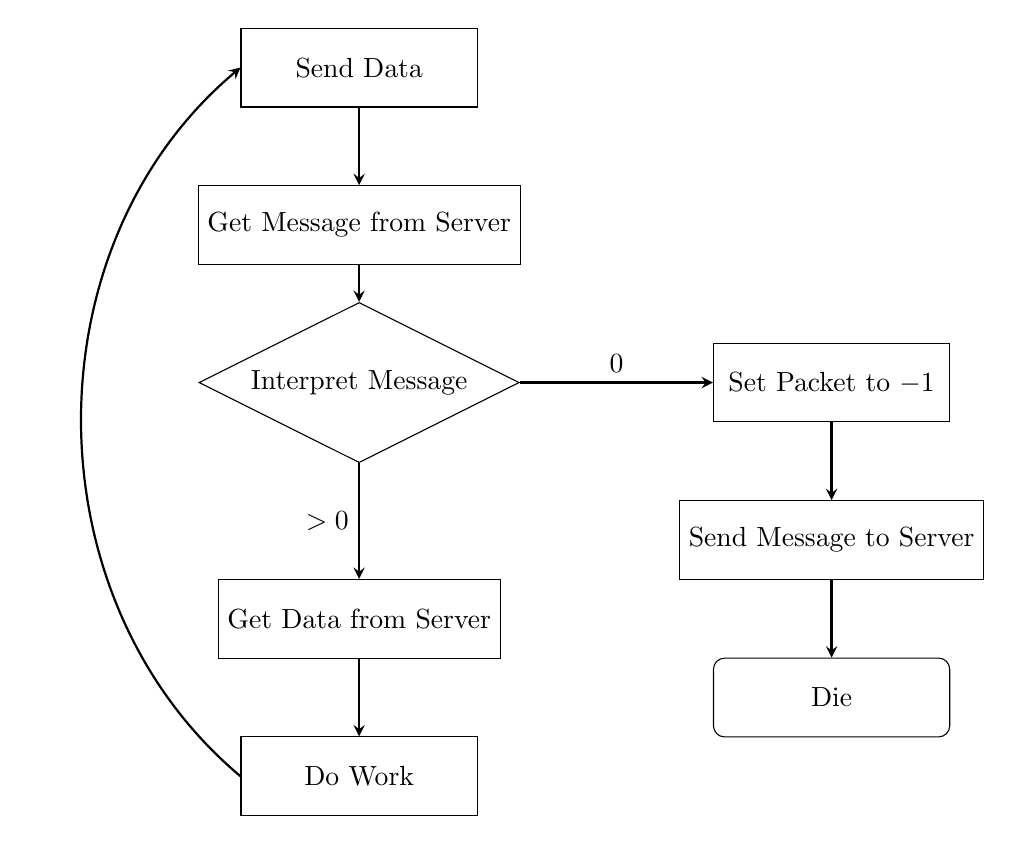
\begin{tikzpicture}[node distance=2cm, tips=proper]
      \node (start)    [process, yshift=-1cm]                    {Send Data};
      \node (getmsg)   [process, below of=start]                 {Get Message from Server};
      \node (interp)   [decision, below of=getmsg]               {Interpret Message};
      \node (getdata)  [process, below of=interp, yshift=-1cm]   {Get Data from Server};
      \node (dowork)   [process, below of=getdata]               {Do Work};

      \node (setmsg)   [process, right of=interp, xshift=4cm]    {Set Packet to \(-1\)};
      \node (sendmsg)  [process, below of=setmsg]                {Send Message to Server};
      \node (end)      [startstop, below of=sendmsg]             {Die};

      \draw [arrow] (start)   -- (getmsg);
      \draw [arrow] (getmsg)  -- (interp);
      \draw [arrow] (interp)  -- node[anchor=east] {\(>0\)} (getdata);
      \draw [arrow] (getdata) -- (dowork);
      \draw [arrow] (dowork.west) edge[bend left=50] (start.west);

      \draw [arrow] (interp)  -- node[anchor=south] {\(0\)} (setmsg);
      \draw [arrow] (setmsg)  -- (sendmsg);
      \draw [arrow] (sendmsg) -- (end);
    \end{tikzpicture}
  \end{figure}

  The flowchart in Figure~\ref{fig:serverflow} shows the decisions and steps the
  server will take in order to distribute the data packets as needed. This 
  flowchart proceeds after the program determines if it's the server or client.
  This flow can be broken down into 3 main parts: the main loop, the wait loop,
  and the program runout.

  The server begins by waiting for a message to come in from a client process.
  If it does not recieve a message, it will go into the wait loop. If it does,
  it will interpet the message it recieves from a client process. The message
  sent to the server can be one of three possible values: \(-1\), \(0\), or an
  integer greater than \(0\). This message serves a dual purpose - to indicate
  the state of the client and to pass along the message size of the data packet
  (if there is one) to be recieved.

  If the server recieves a \(0\), then it has been told that the child has no
  results to send and is waiting for data from the server. If it recieves a
  non-negative value greather than \(0\), it will request the results from the
  client using the message as the size of the data packet to be recieved. In 
  either case, after the server recieves data (if it was sent any),  it will 
  send a packet of size \(n\) to the client to perform work on. This continues
  until there is no more work to be done.

  If the server waits for a client, then it will work on \(\frac{n}{2}\) problems
  before checking to see if it has a message again.

  If the server recieves a \(-1\), then it has been told that the child has
  died after being requested to end, as a confirmation. The server keep track
  of the number of children that have send this message, and when all children
  have died, it will perform the program runout, where it will print out all
  of the solutions that were found.

  As mentioned earlier, \(n\) is the size of packet sent to a client, and can
  be varied. This report will investigate the effect of different sizes of 
  \(n\) has on the runtime and if allowing \(n\) to be freely variable has a
  noticible effect. Additionally, \(n\) gets set to a smaller number when the
  number of remaining games is less than \(n\). Finally, the value of \(n\) can
  be used as a signal to the child that there are no more games available and
  to quit - this occurs when \(n=1\).

  The program uses a na\"{i}ve approach to progressively increasing the size of
  data packet sent to the clients. With exception of when the server recieves a
  message of \(0\) from the client, if the server immediately is given a
  message from a client, it will increment \(n\) by 1 and progressively send
  larger and larger packets to the clients. This is an attempt to ensure that
  the clients are kept busy while the server processes results from clients,
  packages data for clients, and send that data to clients.

  The code as implemented has several command line arguments available to it
  that can vary the initial packet size and allow for packet increment. This
  allows for testing of various scenarios to avoid compiling between runs. By
  default, the program will use an initial packet size of \(n=2\) and will not
  increment the packet.

  The flowchart in Figure~\ref{fig:clientflow} for the client portion is
  relatively straightforward, as the client's main loop is to send data to the
  server, wait for a message from the server, get data from the server, do the
  work, then repeat. During the "Send Data" phase, it will initially send a
  message that contains the message for the server to interpret as outlined
  earlier. Once the client determines that it is a client process, it will
  set this value initally to \(0\). As it recieves data from the server, it
  will set this value to whatever the size of the data it sends to the server.
  Once it has recieved an idication that there is no work to be done, it will
  send back a \(-1\) to the server and quit.

  The flowcharts in both Figure~\ref{fig:serverflow} and 
  Figure~\ref{fig:clientflow} to not take in account for the instance that
  there are \textbf{no} clients (e.g. single-threaded operation). The code as
  implemented has additional escape logic that breaks out of the wait loop when
  the number of games left is 0.

  \section{Analysis}

  The analysis starts with an assumption that in a single-threaded execution,
  approximately 70\% of the execution time is due to finding a solution, as part
  of the execution that will not be parallelized is "playing through" the solved
  games again to output a solution to a text file. This combined with initially
  reading in the file will take some time:

  \[ f = \frac{W_S}{W_S + \sum W_K} = \frac{0.3}{1} = 0.3 \]

  This assumes that \(t_1 = 1\). The upper bound of the speedup, with these
  assumptions is:

  \[ S_{upper} = \frac{1}{f} = \frac{1}{0.3} = 3.\overline{33} \]

  \begin{figure}[t]
    \caption{Estimated Speedup}
    \label{fig:estspeedup}
    \centering

    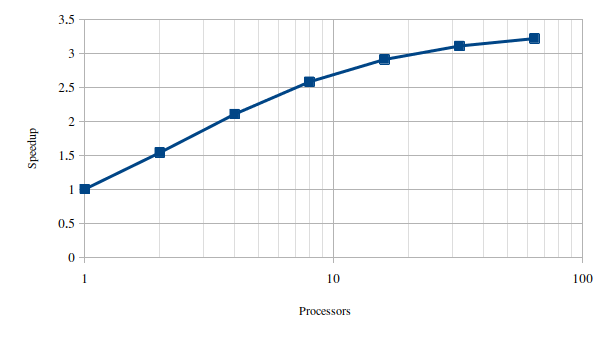
\includegraphics[scale=0.5]{estimatedspeedup}
  \end{figure}

  This is charted in Figure~\ref{fig:estspeedup}.

  Since the estimated speedup falls far short of the ideal speedup, the
  efficiency drops dramatically from 77\% with 2 processors all the way down
  to 5\% with 64 processors. It is not expected that the code will achieve
  superlinear speedup.

  \section{Results}

  84 variations were run 5 times to get a sufficient amount of data to do
  comparisons described earlier in the report: to see the effect of packet size
  on speedup and to see if incrementing the packet size had any effect.

  Initial packet sizes of 1, 2, 10, 25, 50, and 100 were used.

  \begin{figure}[H]
    \caption{Execution Time of Fixed Packet Sizes (Seconds)}
    \label{fig:fixedexectime}
    \centering

    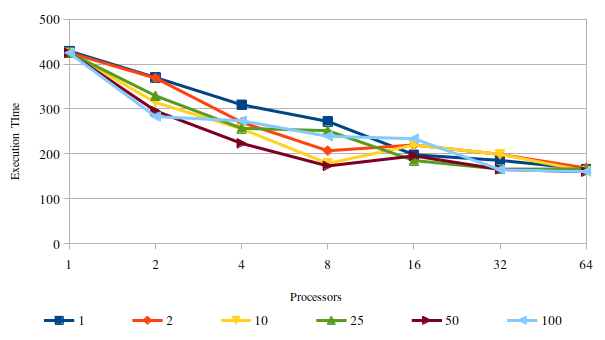
\includegraphics[scale=0.5]{fixedexec}
  \end{figure}

  \begin{figure}[H]
    \caption{Speedup of Fixed Packet Sizes}
    \label{fig:fixedspeedup}
    \centering

    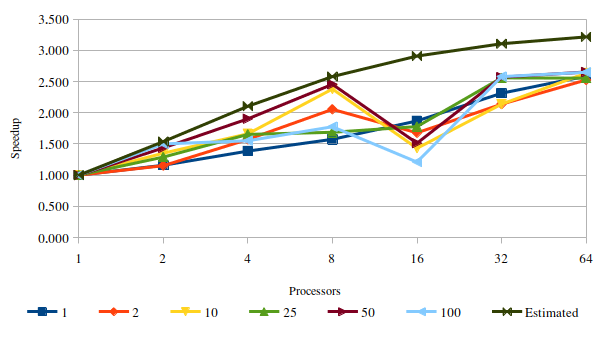
\includegraphics[scale=0.5]{fixedspeedup}
  \end{figure}

  \begin{figure}[H]
    \caption{Execution Time of Dynamic Packet Sizes (Seconds)}
    \label{fig:dynexectime}
    \centering

    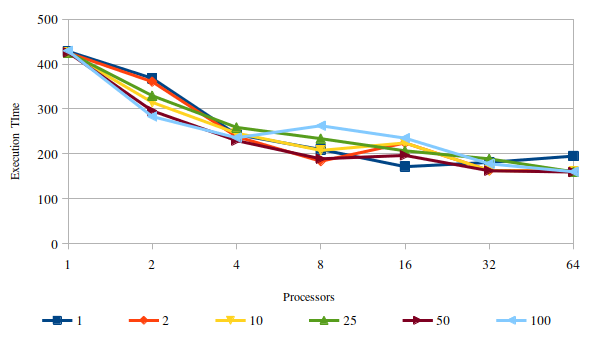
\includegraphics[scale=0.5]{dynexec}
  \end{figure}

  \begin{figure}[H]
    \caption{Speedup of Dynamic Packet Sizes}
    \label{fig:dynspeedup}
    \centering

    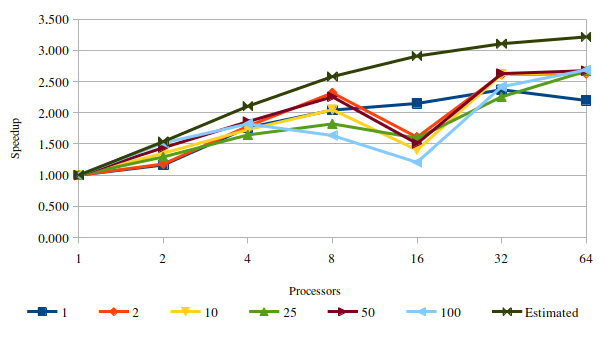
\includegraphics[scale=0.5]{dynspeedup}
  \end{figure}

  \section{Synthesis}

  With exception of the 16 processor runs, nearly every variation of had a 
  speedup close to what was estimated.

  Between the fixed and dynamic packet size runs, the difference is roughly
  negligible, as was the variation between each starting packet size (with
  exception for initial packet size 1 and for runs on 16 processors). Analyzing
  a rough average of the 64 processor run:

  \[ t_1 \simeq 430 seconds \]
  \[ t_64 \simeq 160 seconds \]
  \[ S_{actual} = \frac{430}{160} = 2.688 \]

  This is within bounds of what was estimated speedup would be and is not an 
  unreasonable number. Additionally, the serial fraction is:

  \[ f = \frac{\frac{p}{S}-1}{p-1} = 0.362 \]

  While this is not the initial assumption of the 30\% serial fraction, it is
  not unreasonably wrong.

  The runs using an initial packet size of 1, regardless of being fixed or
  dynamically incremented, seemed to not be affected at 16 processors like the
  other runs.

  \section{Conclusion}

  The actual speedup gained indicated that the initial estimate was not
  unreasonable and that there was not a significant issue with the code. Some
  things that could have been addressed in the analysis was the effect of
  communication costs between processors, as this may have been a contributing
  factor in the error between the estimated speedup and actual speedup.

  Additionally, it seems that dynamically incrementing the packet size had
  little to no effect on speedup, and with exception of the packet size of 1,
  the size of packet had little to no effect as well.

  In the case of a fixed packet size with an initial packet size of 1, it is
  highly likely that client processes are waiting for the server to complete
  its single problem before addressing the needs of the clients. This leads
  to a fairly low speedup overall, though it is not heavily affected past
  8 processors like the other runs. This is perhaps due to cache or overhead
  due to interprocess communications, and the smaller packet size is able to
  avoid these issues.

\end{document}

